\documentclass{article}

\usepackage{amsmath,amssymb,amsthm, amsfonts}   % math
\usepackage{graphicx}   % need for pictures
\usepackage{fullpage}   % makes the margines way smaller
\usepackage{verbatim}
\usepackage{float}
\usepackage{bm}
\usepackage{geometry}
\usepackage{epstopdf}
\geometry{
left=10mm
}

\newcommand{\gj}[9]{ \begin{Bmatrix}
  #1 & #2 & #3 \\
  #4 & #5 & #6 \\
  #7 & #8 & #9
 \end{Bmatrix}}

\newcommand{\Gj}[6]{ \begin{Bmatrix}
  #1 & #2 & #3 \\
  #4 & #5 & #6 
 \end{Bmatrix}}

\newcommand{\tj}[6]{ \begin{pmatrix}
  #1 & #2 & #3 \\
  #4 & #5 & #6 
 \end{pmatrix}}


\title{CHEX Report}
\date{}


\begin{document}

\maketitle
\tableofcontents

\section{Introduction and Motivation for CHEX}

Charge-exchange reactions are isobaric transitions where a proton is converted to a neutron or vice versa.  Examples if these transitions include $(p,n)$ and $(n,p)$ type reactions, as well as reactions involving composite probes, such as $(^3He,t)$ or $(d,pp)$ that explore the same processes.  These reactions can be used to probe a wide variety of applications, including electron capture in supernova, and exploring aspects of exotic nuclear matter.  However, charge-exchange reaction theory is underdeveloped and often relies on a number of assumptions and splifications that restrict the region of validity to higher energies (around 100 MeV/u).  Ideally we would have a more robust theory of charge-exchange reactions, such as in the case of transfer reactions, that allows us to explore a wide variety of energies and angles.  We would also like to explore the efffects of various reaction formalisms and effects from different potentials, including the effects of non-local potentials.  Although there are many charge-exchange reaction codes available, many are legacy codes and were not built with these explorations and expansions in mind.  Therefore, we have decided to build a new code, from scratch, which we are calling CHEX for CHarge-EXchange.  This report is intended to describe the development and implementation of that code.

\section{Formalism}

A full derivation of CHEX is given in another document, but I wanted to briefly describe the formalism we are using.  We are begining with describing $(p,n)$ reactions in the Distorted Wave Born Approximation (DWBA) for fermi transitions.  The problem is cast in a few body framework with an intert core and valance nucleon.  For the case of $(p,n)$ type reactions, the valance nucleon in the incomming channel is a neutron, which becomes a proton in the outgoing channel.  This is shown in Figure \ref{fig:coordinates}.  There are two radial coordinates, $R_{1A}$ which describes the scattering coordinate and $r_{2c}$ which describes the internal coordinate of the target between the core and valance nucleon.

\begin{figure}[H]
	\centering 
    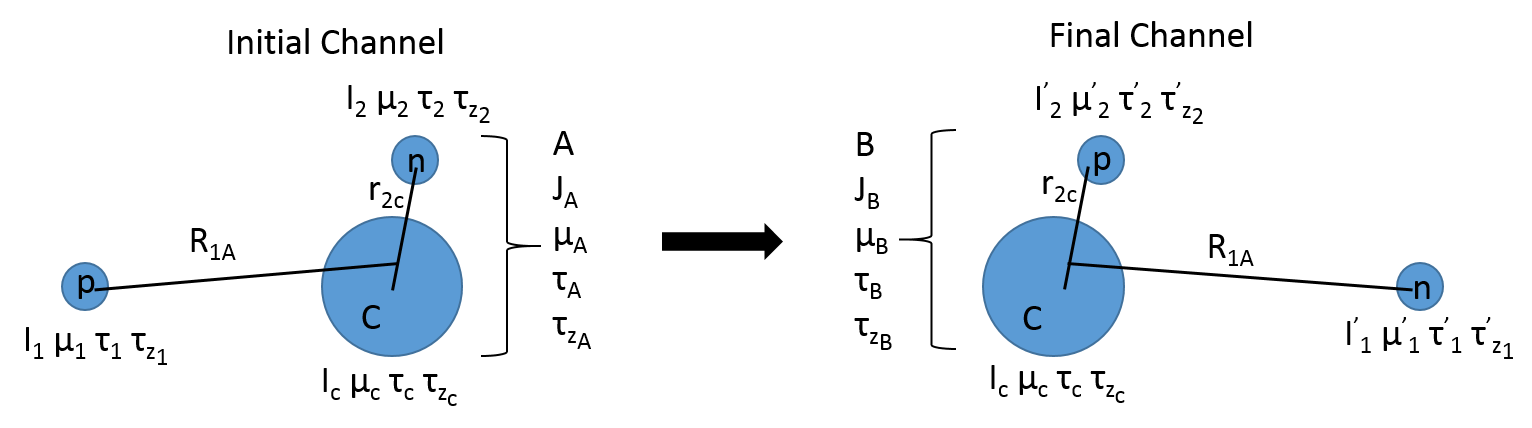
\includegraphics[width=0.7\textwidth]{Coordinates.png}
    \caption{Corodinates and Angular Momentum for the initial and final states of A(p,n)B reaction.}
    \label{fig:coordinates}
\end{figure}

In the most general case, the interaction for charge-exchange can be described as 

\begin{equation} \label{eq:interaction}
t_{NN}=\sum_{i} V(r_{i,p})(1-P_{i,p}) \tau_i \cdot \tau_p
\end{equation}

where the sum runs over the target nucleons, $V(r_{i,p})$ is an NN interaction, $(1-P_{i,p})$ is a term that takes antisymeterization into account, and $\tau \cdot \tau$ is the Fermi operator which changes isospin, but not spin state.  It is worth noting that $r_{i,p}$, which we will refer to as $r_{12}$ is not one of the coordinates chosen for our description of the system, so interactions over this coordinate must be expanded in the $r_{2c}$ and $R_{1A}$ coordinates.

\section{Benchmarking CHEX}

For our first benchmarking case in comparing to work by\cite{Danielewicz2016}.  This work looked at an even simpler subset of charge-exchange reactions, considering only $0^+$ isobaric analogue state (IAS) transitions.  The potential choses was the lane potential whcih is proportional to the difference between a neutron and proton optical model scattering potentials.  The nuclear potentials are parameterized by Koning and Delaroche \cite{KD2003}.  The potentials run over the scattering coordinate ($R_{1A}$), and considers the interaction between the projectile and the entire target, effectively reducing our three-body formalism to a two-body problem.  Also, the sume from  Using the same interaction, we expect to produce the same cross sections for the cases considered by Danielewicz et. al.  Also, in this case, the sum in \ref{eq:interaction} runs over all fo the valance nucleons and leaves us with $\tau_p \cdot \tau_{A}$ for the Fermi operator, where $\tau_A$ is the isospin of the target.

The first step in benchmarking CHEX is to verify that the expression matches the work by Danielewicz for the simlipfied case given above.  A full derivation of my formalism can be seen in the CHEX derivation document.  The final expression for my charge-exchange cross section in the case is given by:

The expression by danielewicz is given by

\begin{equation}\label{eq:Danielewicz1}
\frac{d\sigma}{d\Omega}=\frac{1}{k_p^2} \frac{1}{2s+1} \sum_L (2L+1) A_L^{(p,n)} P_L(cos \theta)
\end{equation}

where $s$ is the spin of a proton, $k_p$ is the wave numberof the incoming proton, and $P_L$ represents the Legendre polynomials.  $ A_L^{(p,n)}$ is given by

\begin{equation}\label{eq:Danielewicz2}
\frac{4}{(\hbar c)^4} \mu_p \mu_n k_p k_n \sum_{J^\prime \ell^\prime} (2J^\prime +1)(2 \ell^\prime +1) \sum_{J \ell}(2J+1)(2 \ell +1) \tj{\ell}{\ell^\prime}{L}{0}{0}{0}^2 \Gj{\ell}{\ell^\prime}{L}{J^\prime}{J}{s}^2 Re[I^*_{J^\prime \ell^\prime} I_{J \ell}]
\end{equation}

where

\begin{equation}\label{eq:Danielewicz3}
I_{J \ell}=2 \frac{\sqrt{|N-Z|}}{A} \int^{\infty}_{0} dr r^2 u^{(+)}_{n,J \ell}(r) U^{J \ell}_1 (r) u^{(+)}_{p,J \ell}(r).
\end{equation}

In this formalism, $\ell$ is the orbital momentum of a given scattering state and $J$ is the total angular momentum of $\ell$ coupled wiith the spin of the projectile.  Because this formalism only describes IAS transitions, the initial orbital momentum is equal to the final orbital momemtum.  $u$ are the radial wavefunctions for the incoming and outgoing channels.  Danielewicz includes the colomb pase factor ($e^{i \sigma_{L_i}}$) and $\frac{1}{k}$ factors in the radial wavefunctions.

Because these two expressions are cast in different forms, it is not straightforward to verify their equivalence.  We used two simple methods: first, I compared the expressions for small L value (i.e. L=0 and L=1) and second, I compared the full expression for all $L$ and $J$ values using mathematica.  

\subsection{Comparing formalism for L=0}

For $L=0$ with the integrals set to 1, Danielewicz et. al.'s expression simplifies to

\begin{equation}
4\frac{k_n}{k_p} \frac{\mu_n \mu_p}{(\hbar c)^4} 
\end{equation}

My L=0 expression with integrals set to 1 gives

\begin{equation}
4\frac{k_n}{k_p} \frac{\mu_n \mu_p}{(\hbar c)^4} \frac{1}{k_n^2 k_p^2}
\end{equation}

The difference can be explained by the fact that Pawel's wavefunctions include the $\frac{1}{k}$ factors, while I write them out explicitly.  Also, it is worth noting that for a long time, my expression was a factor of $4\pi$ less.  This was solved by a missing factor coming from the lagendre polynomials used to expand the potential in my formalism.  With the wave functions and potential set to 1, Danielewicz produces 19824.59 as an $L=0$ solution and CHEX produces 0.0198494.  The $10^6$ difference is because Danielewicz et al. uses GeV as their unit of energy instead of MeV.  

If I then substitute in the $L=0$  wavefunctions (but still set the potential to 1, CHEX obtains the numerical result of 0.432119 and Danielewicz gets the same result, except a factor of $10^6$ larger.


\subsection{Comparing Wave Function}

Because Danielewicz et al includes factors of $k$ and a pseudo-coulomb phase in his wave function calculations, it is not straightforward to show the equivalence of wave functions produced by each code.  The equivalence of the wave functions is shown below for the case of the $L=6$ $J=5.5$ incoming proton scattering wave function for $^{48}Ca(p,n)^{48}Sc$ at 35 MeV/u.  Both the real and imaginary parts of the wave function are shown.  The outgoing wave functions are similarly equivalent but, because there is no coulomb phase for the neutron wave function, the comparison is more clear and is not shown here. 

\begin{figure}[H]
	\centering 
    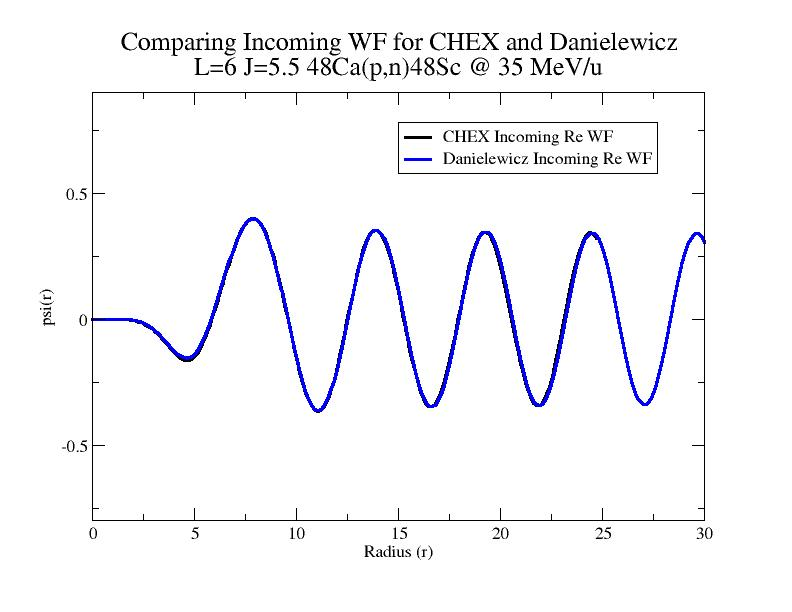
\includegraphics[width=0.7\textwidth]{InWfComp.jpg}
    \caption{Comparing real part of incoming wave functions for CHEX and Danielewicz et al.  This example isfor the L=6, J=5.5 incoming scattering wave function for $^{48}Ca(p,n)^{48}Sc$.}
    \label{fig:inwfcompare}
\end{figure}

\begin{figure}[H]
	\centering 
    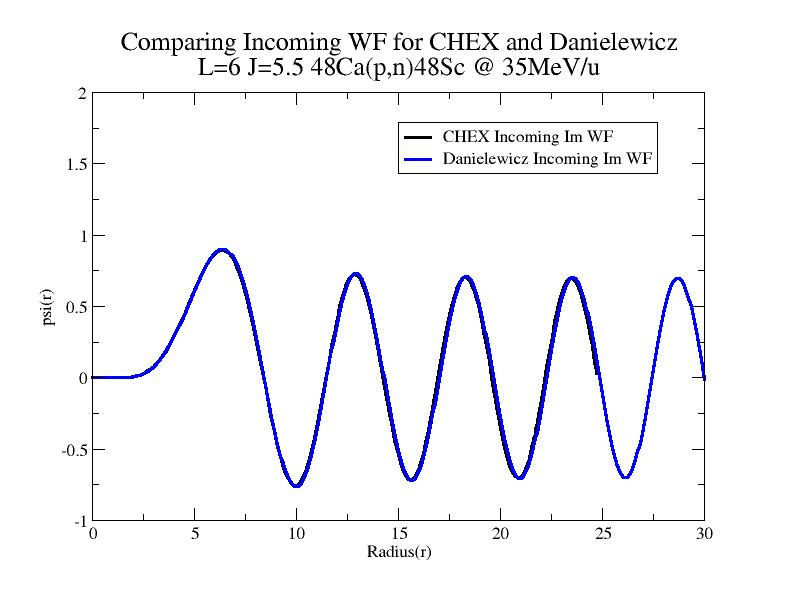
\includegraphics[width=0.7\textwidth]{ImWFComp.jpg}
    \caption{Comparing imaginary part of incoming wave functions for CHEX and Danielewicz et al.  This example isfor the L=6, J=5.5 incoming scattering wave function for $^{48}Ca(p,n)^{48}Sc$.}
    \label{fig:imwfcompare}
\end{figure}

\subsection{Comparing Lane Potential}

We also wanted to prove that we were calucating the Lane potential conistently with Danielewicz et al.  This can be easily done by plotting and comparing the potential.  The below example shows the Lane potential for the $L=4$ $J=3.5$ partial wave in the case of the $^{48}Ca(p,n)^{48}Sc$ reaction.  It is worth noting that Danielewicz uses units of GeV, so his potential was multiplied by a factor of 1000 to compare with CHEX.  Additionally it is worth noting that the Lane potential used in Danielewicz et al (and therefore, CHEX) does not include a coulomb contribution.  The figure below demonstrates that both codes are utilizing an equivalent interaction.

\begin{figure}[H]
	\centering 
    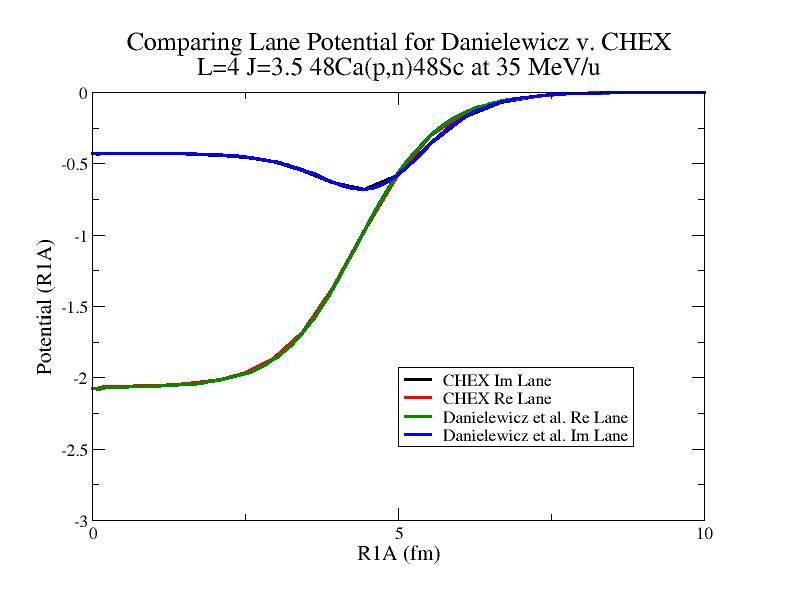
\includegraphics[width=0.7\textwidth]{ComparingLaneFigure.jpg}
    \caption{Comparing the real and imaginary parts of the Lane potential for CHEX and Danielewicz et al.  This example is for the L=4, J=3.5 Lane potential in the for $^{48}Ca(p,n)^{48}Sc$ reaction.}
    \label{fig:imwfcompare}
\end{figure}

\subsection{Comparing Spin 0}

\subsection{Comparing full expression}



\bibliographystyle{plain}
\bibliography{references}

\end{document}